% fig-kokoro-pipeline.tex
% CS1 (Kokoro-82M) decomposed inference pipeline.
% data: surgical-inference.md Section 4.1 (pipeline ASCII diagram) and Section 4.1
%       prose on the shipped staged compute policy + DecoderPre || hn-nsf concurrency.
% Four Core ML model families, three native Swift stages. Per-stage compute-unit
% annotations: DecoderPre = .cpuAndNeuralEngine; Duration, F0Ntrain,
% GeneratorFromHar = .cpuAndGPU; alignment/pad/trim = Swift (CPU).
% Build: tectonic paper/figures/fig-kokoro-pipeline.tex
\documentclass[border=6pt]{standalone}
\usepackage[T1]{fontenc}
\usepackage[scaled]{helvet}
\renewcommand{\familydefault}{\sfdefault}
\usepackage{sansmath}
\usepackage{tikz}
\usetikzlibrary{arrows.meta,positioning,fit,backgrounds,calc}

% Okabe-Ito-derived, colorblind-safe fills; distinct border dash = redundant
% (grayscale-safe) encoding of engine placement.
\definecolor{cmlgpu}{HTML}{CDE4F2}   % Core ML on CPU+GPU  (blue family)
\definecolor{cmlane}{HTML}{C7E9C0}   % Core ML on CPU+ANE  (green family, the ANE stage)
\definecolor{swiftc}{HTML}{FDE3C4}   % native Swift (CPU)  (orange family)
\definecolor{ioblk}{HTML}{E8E8E8}    % I/O endpoints
\definecolor{edgec}{HTML}{444444}

\begin{document}
\sansmath
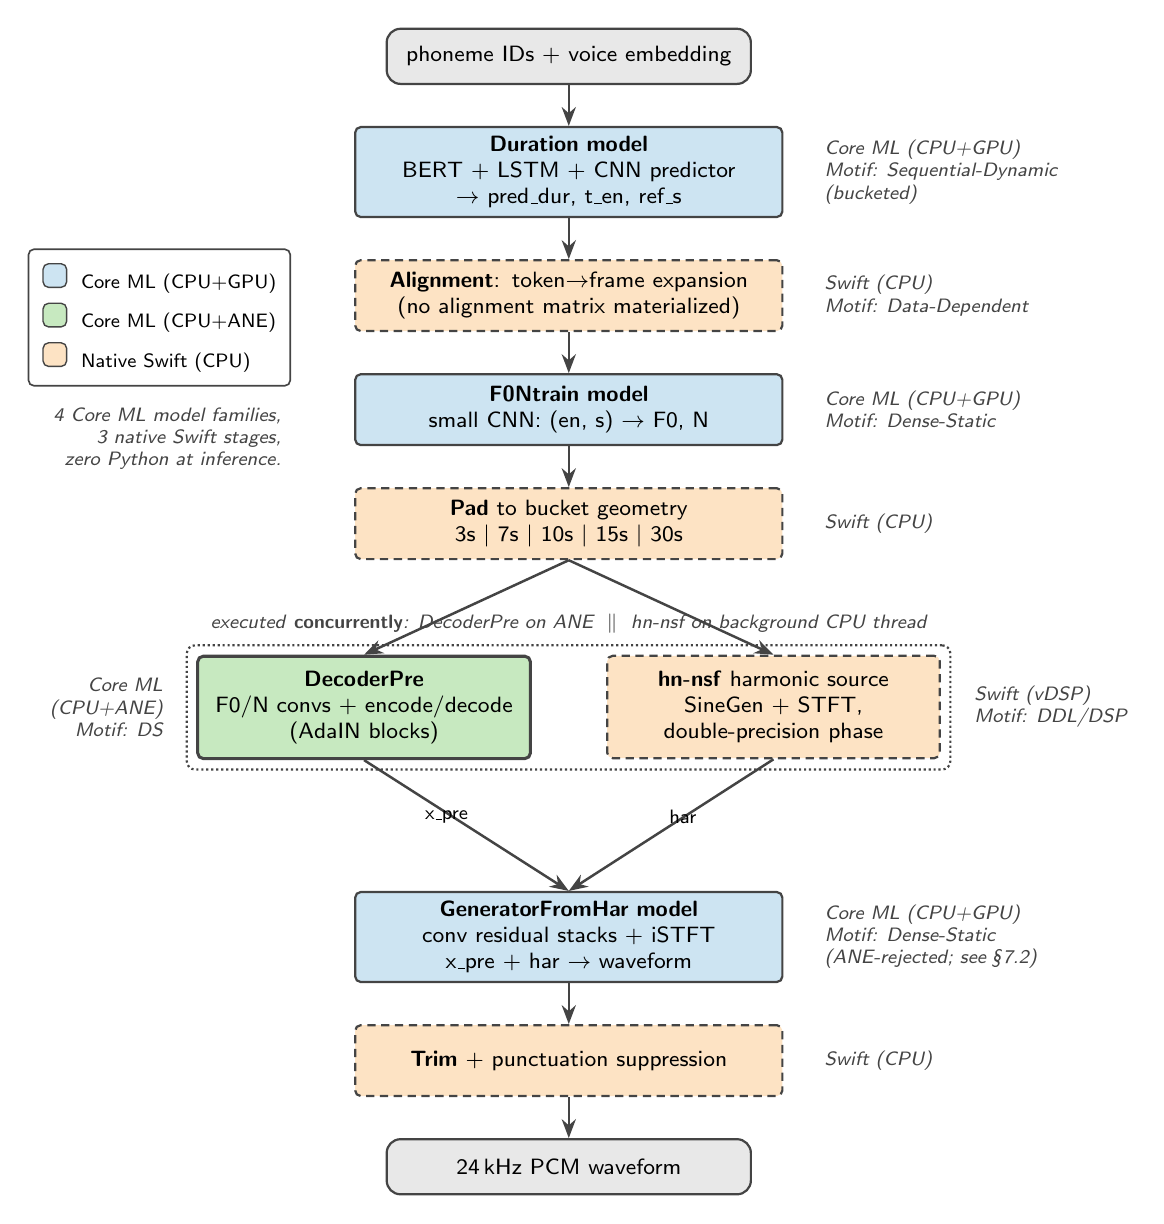
\begin{tikzpicture}[
  font=\sffamily\footnotesize,
  >={Stealth[length=2.4mm]},
  node distance=5.2mm,
  every node/.style={transform shape},
  stage/.style={rectangle, rounded corners=2pt, draw=edgec, line width=0.8pt,
                align=center, inner sep=3.2pt, minimum height=9mm, text width=52mm},
  io/.style={stage, fill=ioblk, draw=edgec, text width=44mm, minimum height=7mm,
             rounded corners=5pt},
  cmlgpu/.style={stage, fill=cmlgpu},
  cmlane/.style={stage, fill=cmlane, line width=1.1pt},
  swiftc/.style={stage, fill=swiftc, densely dashed},
  saned/.style={cmlane, text width=40mm, minimum height=13mm},
  sswift/.style={swiftc, text width=40mm, minimum height=13mm},
  ann/.style={font=\sffamily\scriptsize\itshape, text=edgec, align=left},
  flow/.style={->, draw=edgec, line width=0.9pt},
  swatch/.style={draw=edgec, line width=0.5pt, minimum width=3mm,
                 minimum height=3mm, inner sep=0pt},
]

% ---- main vertical spine ----
\node[io] (in) {phoneme IDs $+$ voice embedding};
\node[cmlgpu, below=of in] (dur)
  {\textbf{Duration model}\\BERT $+$ LSTM $+$ CNN predictor\\$\to$ pred\_dur, t\_en, ref\_s};
\node[swiftc, below=of dur] (align)
  {\textbf{Alignment}: token$\to$frame expansion\\(no alignment matrix materialized)};
\node[cmlgpu, below=of align] (f0n)
  {\textbf{F0Ntrain model}\\small CNN: (en, s) $\to$ F0, N};
\node[swiftc, below=of f0n] (pad)
  {\textbf{Pad} to bucket geometry\\3s $\mid$ 7s $\mid$ 10s $\mid$ 15s $\mid$ 30s};

% ---- concurrent branch ----
\node[saned, below=12mm of pad, xshift=-26mm] (dpre)
  {\textbf{DecoderPre}\\F0/N convs $+$ encode/decode\\(AdaIN blocks)};
\node[sswift, below=12mm of pad, xshift=26mm] (hnsf)
  {\textbf{hn-nsf} harmonic source\\SineGen $+$ STFT,\\double-precision phase};

\node[cmlgpu, below=42mm of pad] (gen)
  {\textbf{GeneratorFromHar model}\\conv residual stacks $+$ iSTFT\\x\_pre $+$ har $\to$ waveform};
\node[swiftc, below=of gen] (trim)
  {\textbf{Trim} $+$ punctuation suppression};
\node[io, below=of trim] (out) {24\,kHz PCM waveform};

% ---- flow edges ----
\draw[flow] (in) -- (dur);
\draw[flow] (dur) -- (align);
\draw[flow] (align) -- (f0n);
\draw[flow] (f0n) -- (pad);
\draw[flow] (pad.south) -- (dpre.north);
\draw[flow] (pad.south) -- (hnsf.north);
\draw[flow] (dpre.south) -- node[pos=0.55, above left=-1pt, font=\sffamily\scriptsize] {x\_pre} (gen.north);
\draw[flow] (hnsf.south) -- node[pos=0.55, above right=-1pt, font=\sffamily\scriptsize] {har} (gen.north);
\draw[flow] (gen) -- (trim);
\draw[flow] (trim) -- (out);

% ---- concurrency bracket ----
\begin{scope}[on background layer]
  \node[draw=edgec, densely dotted, line width=0.8pt, rounded corners=3pt,
        fit=(dpre)(hnsf), inner sep=3.4pt] (conc) {};
\end{scope}
\node[ann, above=0.5pt of conc.north, anchor=south, align=center]
  {executed \textbf{concurrently}: DecoderPre on ANE $\;\parallel\;$ hn-nsf on background CPU thread};

% ---- right-side engine / motif annotations (spine) ----
\node[ann, right=4mm of dur.east]   {Core ML (CPU+GPU)\\Motif: Sequential-Dynamic\\(bucketed)};
\node[ann, right=4mm of align.east] {Swift (CPU)\\Motif: Data-Dependent};
\node[ann, right=4mm of f0n.east]   {Core ML (CPU+GPU)\\Motif: Dense-Static};
\node[ann, right=4mm of pad.east]   {Swift (CPU)};
\node[ann, right=4mm of gen.east]   {Core ML (CPU+GPU)\\Motif: Dense-Static\\(ANE-rejected; see \S7.2)};
\node[ann, right=4mm of trim.east]  {Swift (CPU)};

% ---- branch annotations (outer sides, clear of the joining arrows) ----
\node[ann, left=3mm of dpre, align=right] {Core ML\\(CPU+ANE)\\Motif: DS};
\node[ann, right=3mm of hnsf, align=left] {Swift (vDSP)\\Motif: DDL/DSP};

% ---- legend (compute-unit color key), left of the spine, top open zone ----
\node[anchor=north east, draw=edgec, line width=0.6pt, rounded corners=2pt,
      inner sep=5pt, align=left, font=\sffamily\scriptsize] (leg)
      at ($(align.west)+(-8mm,6mm)$) {%
  {\tikz\node[swatch,fill=cmlgpu]{};}~~Core ML (CPU+GPU)\\[2.5pt]
  {\tikz\node[swatch,fill=cmlane]{};}~~Core ML (CPU+ANE)\\[2.5pt]
  {\tikz\node[swatch,fill=swiftc]{};}~~Native Swift (CPU)};
\node[ann, below=1.5mm of leg.south east, anchor=north east, align=right]
  {4 Core ML model families,\\3 native Swift stages,\\zero Python at inference.};
\end{tikzpicture}
\end{document}
